\section{Introduction}

\subsection{Definition of algorithm}
Following the \emph{Knuth} definition: \emph{an algorithm is a \underline{procedure} which takes and \underline{input}, produces an \underline{output} and is built by a \underline{finite} sequence of \underline{uniquely decodable} and \underline{effective} steps}.

\begin{itemize}
    \item \emph{procedure}, \emph{input $\xrightarrow{}$ output}: basically we are building a function: $ f:I \xrightarrow{} O $ which is also correct $ \forall i \in I $ (this is the biggest difference with AI which have no correctness constraint);
    \item \emph{uniquely decodable}: no ambigual sentences in algorithm description;
    \item \emph{effective}: basic and atomic steps that can be executed in constant time (approximatively small time).
\end{itemize}

\subsection{Method}
We won't use any programming language to avoid syntactic sugar, instead we will use pseudocode and natural language (the less ambigous as possible).

We will build efficient and elegant algorithms to accomplish readability and bug-free means.

Our workflow will follow those steps:
\begin{itemize}
    \item \emph{problem abstraction}: we will go from problem description in natural language to some fancy formalism
    \item \emph{design and analysis}: we will design and analyze a solving algorithm for that problem;
    \item \emph{proof correctness}: we will prove that the proposed algorithm is in fact correct for the problem we are studying;
    \item \emph{experiments}: we will check the correctness and check a posteriori if the prediction made in the analysis phase are in fact correct.
\end{itemize}

\subsection{Von Neumann Model - RAM}
In the past we have been exposed to the Von Neumann model of computation, also know as \emph{Random Access Machine} in which we have read/write of single elements at a time from memory:
\begin{figure}[H]
    \centering
    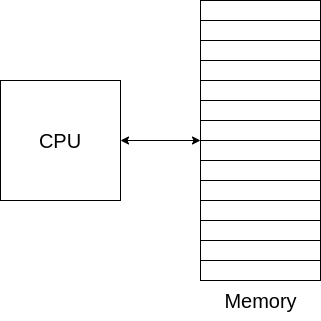
\includegraphics[width=150pt]{images/1_Introduction/RAM_model.png}
    \caption{RAM model}
\end{figure}

In that model of computation the complexity is defined as: 
$$ T_A(n) = \# \text{steps for an input of size } n $$
This definition bring us some problems: we know nothing about the data except the size, if we have any informations about the data we can make better choice on which algorithm to use, moreover the time-complexity is used with asymptotic notation and for worst-case scenario which is not always the case.

\subsection{2-Layer model}
Unluckily Von Neumann architecture is not the case anymore because modern system are built on top of a \emph{memory hierarchy}:
\begin{figure}[H]
    \centering
    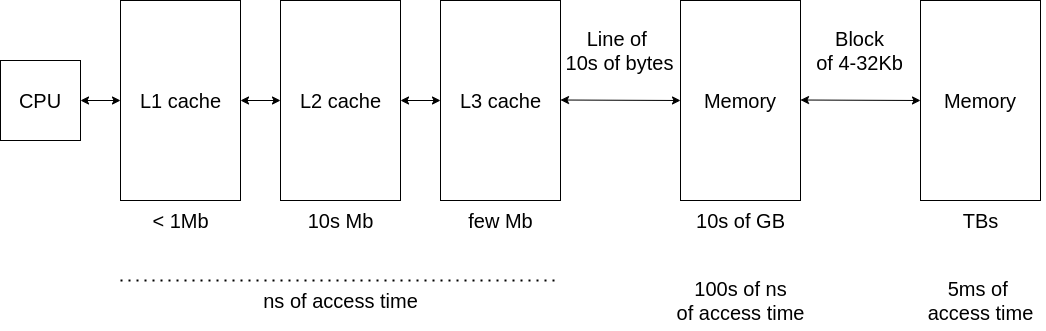
\includegraphics[width=330px]{images/1_Introduction/memory_hierarchy.png}
    \caption{Memory hierarchy}
\end{figure}

Instead of the complex architecture above we will focus on a simpler abstraction:

\begin{figure}[H]
    \centering
    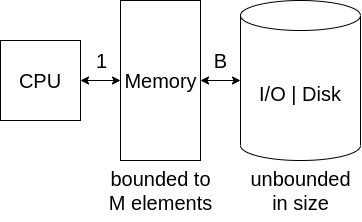
\includegraphics[width=200px]{images/1_Introduction/2-level_model.png}
    \caption{2-layer model}
\end{figure}

In which an access in memory costs 0 and a costs in disk is called \emph{I/O} and that's what we want to estimate.

In this model we try to enforce two properties:
\begin{itemize}
    \item spatial locality: once we have loaded a block from I/O to memory we try to work on all the data on that block before moving on to another one;
    \item temporal locality: is a concept related to the working-set, in fact if it is small probably all my data will fit in memory and once the data has been loaded we won't need more I/O operation.
\end{itemize}
Enforcing these two properties we could diminuish I/O operations, so the time of the algorithm.

\subsection{From time to size}
Let's flip the notation: fixing the time $T$ we want to know how much data we can process.
Let's for example take 3 algorithms:
\begin{itemize}
    \item $T_1(n) = n \implies n \leq T$
    \item $T_2(n) = n^2 \implies n \leq \sqrt{T}$
    \item $T_3(n) = 2^n \implies n \leq \log_2T$
\end{itemize}
Of course the faster the algorithm, the more data we can process, but now we have a relation for data growth on fixed time.
Knowing that relation we can argue on improvements if we improve CPU performance.
Let's for example imagine we buy a $k$ times faster machine, we will get:
\begin{itemize}
    \item $n \leq kT$: improve by $k$
    \item $n \leq \sqrt{kT}$: improve by $\sqrt{k}$
    \item $n \leq \log_2k + \log_2T$: additive improve of $\log_2k$ (additive improve means nothing!)
\end{itemize}


\section{Some examples}
\subsection{Array lookup}
Let's consider a sorted array of integers $A[1 ; n]$, we would like to to search for the element $k$, let's call this procedure $lookup(k)$.

\subsubsection{Scan}
The naivest algorithm is just the linear search. In RAM model it is $O(n)$ cause in the worst case we need to compare each element of the array.

In 2-layer model we need to evaluate the number of I/Os so if we have $B$ elements in each block fetched from the disk we can: start from the left, bring a single block in internal memory and pay 1 I/O, then take the second block and pay 1 I/O and so on and so forth until we find the element inside one block.

In the end we pay $O(\frac{n}{B})$ I/Os in worst case.

\subsubsection{Binary search}
Since the array is sorted in RAM model we can use a binary search, which is $O(log_2 n)$.

In 2-layer model we can almost do the same: fetch the middle block and pay 1 I/O, let's assume we then go to the left, fetch another block paying 1 I/O and so on.
For each jump we pay 1 I/O until we are left with a single block in which the following recursions are free from I/O fetches.
So we do at most $O(log_2 n - log_2 B)$ fetches, which can be written as $O(log_2 \frac{n}{B})$ I/Os.

We can also see it as a binary search in the number of pages, which are of course $\frac{n}{B}$.


\subsection{B+-Tree}
We can further improve the access time using a $B^+-Tree$:
\begin{figure}
    \centering
    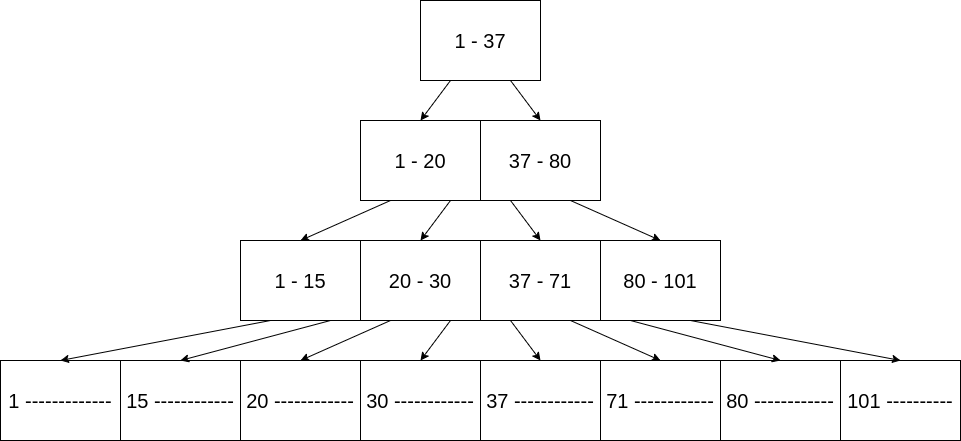
\includegraphics[width=300px]{images/1_Introduction/b+tree.png}
    \caption{B+-Tree}
\end{figure}
The deepest level contains all the values, the next level is formed taking the first element from each block, the next level is built in the same way but starting from the second deepest level, and so on.

The memory occupation is:
\begin{itemize}
    \item $n$ items for the deepest level
    \item $\frac{n}{B}$ for the second level
    \item $\frac{n}{B^2}$ for the next level
    \item ...
    \item $\frac{n}{B^i}$ for the $i$-th level
\end{itemize}
We build levels until we reach a level in which we have a single block, that happens when:
$$
    \frac{n}{B^i} \leq B \implies n \leq B^{i+1}
$$
so we can estimate the tree steep via:
$$
    log_B(n) \leq i+1 \implies i \geq log_B(n) + 1
$$
So we basically built a $B$-ary tree.

To search we start from the root, we bring that root block in memory and perform a search inside it to find the interval, then we fetch the next block and so on.
We fetch a block for each level so $O(log_Bn)$ I/Os.
It's a huge improvement!

\subsubsection{In RAM model}
Let's consider the traversal in RAM model: for each of the $O(log_Bn)$ I/O fetch we need to perform a binary search inside the block so in the end we have:
$$
    log_B n \cdot log_2 B = \frac{log_2 n}{log_2 B} \cdot log_2 B = log_2 n
$$

\subsubsection{Example}
Let's consider those data: $n=2^{30}$, $B=32Kb$, 8 bytes of key and 8 bytes for the pointers:
\begin{itemize}
    \item each page has $\frac{32kb}{16} = 2000$ values inside, which is the fan-out of the tree
    \item we pay $log_{2000} 2^{30} = \frac{log_2 2^{30}}{log_2 2000} \approx \frac{30}{10} = 3$
    \item with binary search we would have paid $log_2 \frac{2^{30}}{32Kb} = log_2 2^{15} = 15$
\end{itemize}

\subsection{Sum of n integers}
We have an array of integers $A[1;n]$ with $n$ very large and $A$ is stored on disk (we mean GBs or TBs of data) and we want to perform the sum of all the values inside $A$.

\subsubsection{Linear Scan}
The naivest approach is to use the scan algorithm , we iterate over the single blocks from left to right and we sum all the values inside the blocks.
It's I/O complexity is $O(\frac{n}{B})$, it's an optimal algorithm because we can't do better since we need to access every item at least once.

\subsubsection{Jump Scan}
Let's think about another algorithm which jumps around to access items. Let's call it $Alg_{s,b}$ in which $s$ is how much we jump each time and $b$ is the block size of the algorithm, so the number of elements we process for each jump.
So we have blocks of size $B$ splitted in smaller blocks with size $b$ (assume $b$ divides $B$).

Our algorithm is:
\begin{itemize}
    \item start from a block (of size $b$), sum all the items
    \item jump $s$ blocks far away and start again until the end
\end{itemize}

Let's analyze the algorithm: the $j$-th block is $A[j \cdot b + 1; (j+1) \cdot b]$ with $j=0, 1,_,\frac{n}{b}-1$, let's use $i$ to point to the block to process: $j = s \cdot i \mod \frac{n}{b}$ with $i=0, 1,_, \frac{n}{b}-1$ ($j$ is a permutation if and only if $s$ and $\frac{n}{b}$ are coprime, so let's assume it).
This definition of $i$ and $j$ says that we scans all blocks and we loop over them just once but:
\begin{itemize}
    \item increasing $s$ decreases locality because we process less elements at each jump
    \item increasing $b$ increases locality because smaller blocks means smaller jumps
\end{itemize}

We have some edge cases:
\begin{itemize}
    \item $s=1$, $b$ is whatever: we have the scan algorithm
    \item $s>1$, $b=1$: is the worst since we process a single element and then jump
\end{itemize}

Analyzing them from RAM model point of view those algorithms are all equivalent but in 2-layer models they are not.
Let's assume $b \leq B$ and $s=2$: we will exploit half of the blocks per page so we need a second pass to compute a full page!

In the end the number of passes is $s$ if $s < \frac{B}{b}$ so the I/O complexity is $O(\frac{n}{B} \cdot min\{s, \frac{n}{B}\})$

\section{Virtual Memory}
Let's assume we have $M$ items in memory and $(1+\epsilon)\cdot M$ elements on disk ($M$ elements are both on disk and in memory).
We want to calculate the probability that my algorithm will access the disk:
$$
    P(\epsilon) = \frac{\epsilon \cdot M}{(1+\epsilon)\cdot M} = \frac{\epsilon}{1+\epsilon}
$$
That calculation is for a completely random algorithm which is not reasonable.

We can have a better estimation using some empiric data:
\begin{itemize}
    \item we read/write not in constant time for $a \approx 30\%$
    \item we compute in constant time for $1-a \approx 70\%$
    \item assume $C$ as the cost of an I/O operation
\end{itemize}
The average cost of a step is:
$$
    (1-a)O(1) + a[P(\epsilon) \cdot C + (1-P(\epsilon))\cdot O(1)] \approx a \cdot P(\epsilon) \cdot C
$$

\subsection{Example}
Assuming:
\begin{itemize}
    \item access in memory is $O(1) \approx 100ns = 10^{-7}s$
    \item access to disk is $5ms = 5 \cdot 10^{-3}s$
    \item $C = \frac{5 \cdot 10^{-3}}{100 \cdot 10^{-9}} = 5 \cdot 10^4$
\end{itemize}
the average cost of an operation is: $0.3 \cdot \frac{1}{1000} \cdot 5 \cdot 10^4 = 15$.

The more the gap between memory and disk, the more the average cost, they are linearly dependant.



